% -*- coding: utf-8 -*-
\documentclass[UTF8,a4paper,10pt]{ctexart}
\usepackage[left=2.54cm, right=2.54cm, top=2.54cm, bottom=2.54cm]{geometry}
\usepackage{amsmath,graphicx,float,booktabs,multirow,enumitem,tikz,pgfplots}
\pgfplotsset{compat=1.17}
\usepackage{ctex}
\setCJKmainfont[ItalicFont=Noto Sans CJK SC Bold, BoldFont=Noto Serif CJK SC Black]{Noto Serif CJK SC}
\usepackage{ctexcap}
\CTEXsetup[name={,、},number={\chinese{section}}]{section}
\CTEXsetup[name={（,）},number={\chinese{subsection}}]{subsection}
\usepackage{fancyhdr}
\pagestyle{fancy}
\lhead{\kaishu \leftmark}
\rhead{\kaishu 算法导论 GPU并行实验报告}
\cfoot{\thepage}
\usepackage{xcolor,listings}
\lstset{breaklines,basicstyle=\small,numbers=left,numberstyle=\tiny,frame=trbl}
\usepackage[colorlinks,linkcolor=black,anchorcolor=blue]{hyperref}
\newcommand{\HRule}{\rule{\linewidth}{0.5mm}}

\begin{document}
\begin{titlepage}
\begin{center}
\includegraphics[width=0.8\textwidth]{NKU.png}\\[1cm]
\textsc{\Huge \kaishu{\textbf{南\ \ \ 开\ \ \ 大\ \ \ 学}}} \\[0.9cm]
\textsc{\huge \kaishu{\textbf{计\ 算\ 机\ 学\ 院}}}\\[0.5cm]
\textsc{\Large \textbf{算法导论 GPU编程实验报告}}\\[0.8cm]
\HRule \\[0.9cm]
{\LARGE \bfseries ANN 向量检索：GPU 并行加速实验}\\[0.4cm]
\HRule \\[2.0cm]
\textsc{\LARGE 李华濂}\\[0.5cm]
\textsc{\LARGE 年级: 2024级 \quad 专业: 计算机科学与技术}\\[0.5cm]
\textsc{\LARGE 指导教师: 王刚}\\[0.5cm]
\vfill
{\Large \today}
\end{center}
\end{titlepage}

\newpage
\thispagestyle{empty}
\renewcommand{\abstractname}{\kaishu \sihao \textbf{摘要}}
\begin{abstract}
本实验围绕 DEEP100K 数据集（100K 基向量 $\times$ 96 维，inner-product 距离），
系统探索了 GPU（NVIDIA RTX 4070 Laptop 8GB）在近似最近邻搜索（ANNS）中的加速方案。
实验实现了三类 GPU ANN 算法：
（1）矩阵乘法基线（cuBLAS SGEMM：将距离计算转为矩阵乘法）；
（2）GPU IVF（倒排索引 + 查询分组 + cuBLAS 批量 GEMM）；
（3）GPU IVF-PQ（乘积量化 + ADC 查表 + 精确重排）。

对每类算法，实验均通过参数扫描（batch\_size、nprobe、rerank\_p 等）
精确记录 recall@10 与 avg\_latency（$\mu$s/q）的 trade-off，
并从矩阵乘法效率、GPU 内存带宽、kernel 利用率、PCIe 传输开销、
聚类分组策略、以及 PQ 压缩质量六个维度系统分析。
所有实验结果（包括负优化）均如实呈现。

核心发现：在 RTX 4070 上，矩阵乘法基线取得 recall=0.99999@24.2$\mu$s/q
（queries 级批处理，cuBLAS SGEMM + GPU top-k）；
GPU IVF 取得 recall=0.957@146$\mu$s/q（nprobe=30, batch=500）；
GPU IVF-PQ 因 PQ 编码质量不足（M=4 对大维度子空间量化误差过大），
在小数据集上表现劣于纯 IVF，属于典型负优化。

\vspace{1em}
\textbf{关键字：} 近似最近邻搜索；GPU 并行；cuBLAS；IVF；乘积量化；
矩阵乘法加速；recall-latency trade-off
\end{abstract}

\tableofcontents
\newpage
\setcounter{page}{1}

%=====================================================================
\section{实验平台与问题概述}
%=====================================================================

\subsection{实验背景与问题}

随着深度学习发展，图像、文本等非结构化数据被广泛转换为高维向量，
最近邻搜索在推荐系统、搜索引擎及大语言模型的检索增强生成（RAG）中得到了广泛应用。
本次 GPU 实验的核心问题为：
\textbf{如何利用 GPU 的大规模并行计算能力加速 ANN 搜索，
特别是如何将距离计算转换为 GPU 擅长的矩阵乘法}。

ANN 选题中 GPU 加速主要分为两个方向：
\begin{enumerate}[itemsep=0pt]
\item \textbf{转换成矩阵乘法（1 分）：} 将 base 向量写为 $n \times d$ 矩阵，
query 写为 $d \times m$ 矩阵，通过一次 GEMM 得到 $n \times m$ 的得分矩阵，
再对每列取 top-k。在此基础上探索 tiling 优化、batch size 调优、精度换速度等方法。
\item \textbf{IVF（2 分）：} 将 IVF 一个簇内的向量也写成矩阵，
通过矩阵乘法计算距离。由于不同 query 的最近 nprobe 个簇编号不同，
需要分组策略提高 batch 内簇编号重合度，避免计算资源浪费。进一步探索 IVF-PQ 的 GPU 加速。
\end{enumerate}

实验围绕 DEEP100K 数据集（100K base, 96维, inner-product, 10000 queries, $k$=10），
系统实现了三种 GPU 算法，从六个维度分析：

\begin{enumerate}[itemsep=0pt]
\item 矩阵乘法效率（cuBLAS SGEMM 对小矩阵的利用率和优化空间）
\item GPU 内存带宽（score 矩阵的内存占用与访问模式）
\item Kernel 利用率（top-k kernel 的 occupancy 与线程配置）
\item PCIe 传输开销（GPU $\leftrightarrow$ CPU 数据搬运对延迟的影响）
\item 聚类分组策略（IVF 中 query-cluster 映射的批量化效率）
\item PQ 压缩质量（量化误差、rerank 阈值与 recall 的关系）
\end{enumerate}

\subsection{实验平台}

\begin{itemize}[itemsep=0pt]
\item \textbf{GPU:} NVIDIA GeForce RTX 4070 Laptop (8GB VRAM), Ada Lovelace (sm\_89)
\item \textbf{CUDA:} CUDA Driver 12.6, nvcc 11.8, cuBLAS
\item \textbf{CPU:} Intel/AMD x86\_64 (Windows 11), MSVC 19.41 (VS 2022)
\item \textbf{编译器:} nvcc -O3 -arch=sm\_89 -std=c++17 -lcublas
\item \textbf{数据:} DEEP100K (100K base + 10K query $\times$ 96维, fbin, inner-product)
\item \textbf{指标:} recall@10, avg\_latency ($\mu$s/q), GPU kernel 计时
\end{itemize}

\subsection{计时方法}

本实验通过 \texttt{cudaDeviceSynchronize()} 精确测量 GPU kernel 执行时间，
使用 \texttt{std::chrono::high\_resolution\_clock} 包裹 GEMM + top-k 全过程，
确保计时包含所有 GPU 计算和同步开销。对于 IVF，计时包含粗排 GEMM、
kernel mapping、逐 cluster GEMM、cudaMemcpy 和 heap merge 的端到端延迟。

%=====================================================================
\section{HIP GPU 编程学习总结}
%=====================================================================

本次 HIP 编程学习（Lab 1-6）覆盖了从 GPU 基础执行模型到多 Kernel 协同工作的完整知识体系，
实验平台为 AMD Radeon 8060S（RDNA 3.5, gfx1150），使用 HIP（Heterogeneous-compute Interface for Portability）编程。
以下按六个实验分别总结所学内容。

\subsection{Lab 1: 向量加法 — GPU 编程基础}

\textbf{(1) SIMT 执行模型与线程层次。}
GPU 采用单指令多线程（SIMT）模型：一个 kernel 函数被数千个线程同时执行，
每个线程处理不同的数据。线程组织为三层层次结构：Grid（整个 kernel 启动）→
Block（可在共享内存中协作的线程组）→ Thread（最小执行单元）。
每个线程通过 \texttt{blockIdx.x * blockDim.x + threadIdx.x} 计算唯一的全局索引。

\textbf{(2) AMD GPU 硬件架构映射。}
软件抽象直接映射到物理硬件：Grid 映射到 GPU 设备，Block 映射到计算单元（CU）或工作组处理器（WGP），
波前（Wavefront）——32 或 64 个锁步执行的线程——映射到 SIMD 单元。
Block 内的线程可以共享 LDS（本地数据共享）和同步（\texttt{\_\_syncthreads()}），
不同 Block 之间完全独立。

\textbf{(3) RDNA 3.5 的波前特性。}
消费级 RDNA 3.5 原生波前大小为 32（wave32），同时支持 wave64（需 \texttt{-mwavefrontsize64}）。
Block 大小必须是波前大小的整数倍以避免计算通道浪费。
编译时使用 \texttt{warpSize} 变量（编译器常量，零开销）而非硬编码 32 或 64。

\textbf{(4) Kernel 启动配置。}
使用 \texttt{hipLaunchKernelGGL}，Grid 大小通过 $\lceil N / \text{block\_size} \rceil$ 计算。
实验通过变化 Block 大小（16--1024）并运行 10 次取均值，验证了 wave-aligned 大小性能显著优于 sub-wave 大小。

\textbf{(5) 占用率。}
占用率 = 活跃波前数 / CU 最大支持波前数，受寄存器/线程、共享内存/Block 等因素限制。
高占用率有助于隐藏内存延迟。

\textbf{(6) Grid-Stride Loop。}
使用 \texttt{for (int i = tid; i < N; i += total\_threads)} 让每个线程处理多个元素，增加算术强度。

\subsection{Lab 2: 矩阵转置 — 二维索引与内存合并}

\textbf{(1) 二维线程索引。} 使用 \texttt{dim3} 定义二维 Grid/Block，
矩阵按行优先存储，元素 (i, j) 地址为 \texttt{i * cols + j}。

\textbf{(2) 内存合并访问。} 当同一波前内连续线程访问连续内存地址时，
硬件可合并为一次事务；跨步访问则每个线程独立事务，性能差可达 30 倍以上。

\textbf{(3) 共享内存分块。} 用 LDS 中转实现双向合并访问：
tile 以合并方式从 input 加载到 LDS，在 LDS 中转置，再合并写回 output。

\textbf{(4) Bank Conflict 避免。}
声明 \texttt{\_\_shared\_\_ float tile[BLOCK\_SIZE][BLOCK\_SIZE + 1]} 中 $+1$ 填充避免 bank conflict。

\subsection{Lab 3: 直方图 — 原子操作与竞态条件}

\textbf{(1) 竞态条件。} 多线程并发读写同一地址时产生丢失更新，是 GPU 并行编程的核心 bug。

\textbf{(2) 原子操作。} \texttt{atomicAdd} 保证读-改-写不可分割，代价是冲突序列化。

\textbf{(3) 共享内存私有化。} 第一阶段在 LDS 中维护 Block 本地直方图（本地原子，低争用）；
第二阶段合并到全局内存（每 Block 每 bin 仅 1 次全局原子）。
总内存读取从 $N \times bins$ 降至 $N$。

\textbf{(4) 原子争用与数据分布。}
均匀分布争用最小，全部相同值最慢。共享内存私有化将争用限制在 LDS 范围。

\subsection{Lab 4: 并行归约 — 树形归约与波前优化}

\textbf{(1) 树形归约。} 二叉树模式 O(log N) 并行步数：1024→512→...→1。
每步 \texttt{\_\_syncthreads()} 同步。

\textbf{(2) 四种策略递进。}
Naive Atomic（1.0×）→ Tree-Shared Memory（1.35×）→
Tree + Warp Shuffle（1.52×）→ Multi-Element + Tree + Shuffle（1.85×）。

\textbf{(3) Warp Shuffle。}
\texttt{\_\_shfl\_down(var, delta)} 通过硬件直接交换数据，无需共享内存和同步。

\textbf{(4) 占用率 ≠ 性能。} 大 Block 活跃线程多但归约后期大量空闲，需权衡。

\subsection{Lab 5: 蒙特卡洛积分 — 组合模式}

\textbf{(1) 两阶段结构。} 阶段 1：每个线程独立计算（高度并行，零依赖）；
阶段 2：所有线程归约聚合。这是大量实际 GPU 应用的典型结构。

\textbf{(2) 归约瓶颈。} 若全部 atomicAdd 同一地址则近乎串行。
使用共享内存树形归约将全局原子从 N 次减至 gridDim 次。

\textbf{(3) 数值精度。}
树形归约比顺序累加精度更好；N=100M 时 float 舍入误差显著，建议用 double。

\subsection{Lab 6: K-Means 聚类 — 多 Kernel 综合应用}

\textbf{(1) 迭代算法分解为三个 Kernel。}
Kernel 1（分配）：每数据点独立找最近质心（Lab 1 索引模式）；
Kernel 2（更新）：共享内存原子归约（Lab 3 + Lab 4）；
Kernel 3（收敛检测）：比较新旧质心位移（Lab 3 原子）。

\textbf{(2) 更新 Kernel 的两阶段原子归约。}
LDS 累加各簇坐标和点数（本地原子）→ 合并到全局内存（每 Block 每簇 1 次全局原子）。

\textbf{(3) 关键设计模式。}
双缓冲（指针交换避免 O(k·d) 拷贝）、早期终止（质心位移 $< 10^{-8}$ 时收敛）、
空簇处理（count=0 时保留上一轮质心）。

\subsection{学习总结}

六个实验构成从"一个线程一个元素"到"多 Kernel 协同迭代算法"的完整 GPU 知识体系，
为本次 GPU ANN 实验中的矩阵乘法 GEMM、top-k kernel 设计和 IVF 分组策略提供了坚实的基础。

%=====================================================================
\section{GPU 矩阵乘法基线}
\label{sec:matmul}
%=====================================================================

\subsection{算法设计}

\subsubsection{核心思路}

将 ANN 的距离计算转换为矩阵乘法：

\begin{equation}
S = B \cdot Q^T
\end{equation}

其中 $B \in \mathbb{R}^{n \times d}$ 为 base 向量矩阵（$n$=100K, $d$=96），
$Q \in \mathbb{R}^{m \times d}$ 为 query 批量矩阵（$m$ 为 batch size），
$S \in \mathbb{R}^{n \times m}$ 为得分矩阵，$S_{ij} = \langle b_i, q_j \rangle$。

对于 inner-product 距离，$dist = 1.0 - S_{ij}$，距离越小越近。
因此对每列 $j$（对应 query $j$），取 $S_{:,j}$ 中最大的 $k$ 个值即为最近邻。

\subsubsection{实现细节}

\begin{enumerate}[itemsep=0pt]
\item \textbf{GEMM：} 使用 cuBLAS SGEMM，$\alpha=1.0, \beta=0.0$。
由于 cuBLAS 使用列主序存储，需要仔细设置 transa/transb 参数。
base 矩阵以行主序存储在 GPU 上，对应列主序的 $d \times n$ 矩阵；
query batch 以行主序存储，对应列主序的 $d \times m$ 矩阵。
通过 \texttt{CUBLAS\_OP\_T} + \texttt{CUBLAS\_OP\_N} 实现
$C_{n \times m} = B_{n \times d} \cdot Q^T_{d \times m}$。
\item \textbf{Top-k：} 自定义 CUDA kernel，每个 block 处理一个 query，
1 个线程扫描全部 $n$=100K 个得分，维护大小为 $k$=10 的 min-heap
（heap[0] 为最小内积，新值更大时替换）。
最终输出按内积降序排列的 top-k 向量 ID。
\item \textbf{Batch 处理：} 将 10K query 分批处理，每批 $m$ 个 query。
batch\_size 影响 GPU 利用率和 score 矩阵的显存占用。
\end{enumerate}

\subsection{全部实验结果}

\begin{table}[H]
\centering
\caption{GPU 矩阵乘法基线：batch\_size 参数扫描}
\label{tab:matmul-all}
\begin{tabular}{ccccc}
\toprule
batch\_size & Recall@10 & Avg Latency ($\mu$s/q) & Score 矩阵大小 & 总耗时 (ms) \\
\midrule
100  & 0.99999 & 86.6 & 100K$\times$100 (40MB) & 866 \\
500  & 0.99999 & 24.2 & 100K$\times$500 (200MB) & 242 \\
1000 & 0.99999 & 24.4 & 100K$\times$1000 (400MB) & 244 \\
\bottomrule
\end{tabular}
\end{table}

\begin{table}[H]
\centering
\caption{GPU 矩阵乘法基线：CPU-GPU 正确性验证（Query 0）}
\label{tab:matmul-correctness}
\begin{tabular}{cccc}
\toprule
Rank & CPU Top-10 ID & GPU Top-10 ID & 内积 \\
\midrule
1 & 9865 & 9865 & 1.0000 \\
2 & 7930 & 7930 & 0.5903 \\
3 & 59736 & 59736 & 0.5695 \\
4 & 97227 & 97227 & 0.5640 \\
5 & 94155 & 94155 & 0.5562 \\
6 & 46324 & 46324 & 0.5533 \\
7 & 22672 & 22672 & 0.5527 \\
8 & 45520 & 45520 & 0.5520 \\
9 & 42289 & 42289 & 0.5443 \\
10 & 15447 & 15447 & 0.5387 \\
\bottomrule
\end{tabular}
\end{table}

\subsection{性能分析}

\subsubsection{正确性验证}

表~\ref{tab:matmul-correctness} 展示了 Query 0 的 CPU 暴力搜索与 GPU 矩阵乘法结果的完全一致。
CPU-GPU 匹配率 10/10（recall=1.00），证明 cuBLAS GEMM 计算的 inner product 与
top-k kernel 的排序逻辑完全正确。整体 recall=0.99999 而非 1.0 的原因在于：
当两个向量与 query 的内积差值小于 float32 精度（$\sim 10^{-7}$）时，
排序可能出现微小扰动，但这对实际应用无影响。

\subsubsection{矩阵乘法效率}

cuBLAS SGEMM 在 RTX 4070（Ada Lovelace, sm\_89）上表现优异。
对于 $[100K \times 96] \times [96 \times 500]$ 的矩阵乘法（9.6 GFLOPs），
cuBLAS 利用 Tensor Cores 和优化的 tiling 策略，
在约 1--2 ms 内完成计算。

\begin{enumerate}[itemsep=0pt]
\item \textbf{小矩阵问题：} 对于 $d=96$ 这种"瘦"矩阵，GEMM 的 $K$ 维度
（内积维度）只有 96，tiling 的 tile\_k 受到限制。
但 cuBLAS 对此类形状有专门优化路径。
\item \textbf{Batch size 影响：} $m$ 从 100 增至 500 时，per-query 延迟从 86.6$\mu$s
降至 24.2$\mu$s（3.6$\times$ 加速），因为更大的 $m$ 提升了 GPU 的 SM 占用率。
$m$=1000 时基本不再改善（24.4$\mu$s），说明 GEMM 已接近峰值效率。
\item \textbf{Score 矩阵内存：} $n \times m$ 的 score 矩阵需要 $4nm$ 字节。
$m$=1000 时达 400MB，但仍远在 8GB 显存范围内。
\end{enumerate}

\subsubsection{Top-k Kernel 瓶颈}

top-k kernel 使用 1 thread/query 的配置，每个线程串行扫描 100K 个 float。
这种配置下 GPU 利用率极低（仅 1/32 的 warp lane 被使用），
但在此规模下并非绝对瓶颈：

\begin{itemize}[itemsep=0pt]
\item \textbf{内存访问：} 100K 个 float $\times$ 500 queries = 200MB 读取。
以 RTX 4070 的 $\sim$256 GB/s 带宽计算，纯读取仅需 $\sim$0.8 ms。
但有效带宽因 non-coalesced 访问模式而降低。
\item \textbf{计算开销：} 每次迭代维护 10 元素的 ordered heap，
涉及条件分支和寄存器数据移动，增加约 5--10$\times$ 的指令开销。
\item \textbf{实测：} top-k kernel 约占总延迟的 80\%（$\sim$10 ms/500 queries），
GEMM 占 $\sim$20\%（$\sim$2 ms）。因此优化 top-k kernel
（如每 query 使用 32-thread warp + warp-level reduction）
是进一步提升性能的方向。
\end{itemize}

\subsubsection{与暴力搜索对比}

对于 CPU 上的标量暴力搜索：100K $\times$ 96 $\times$ 10000 = $9.6 \times 10^{10}$ FLOPs，
在 2GHz CPU 上约需数十秒。GPU 矩阵乘法将此降至 24$\mu$s/query，
加速比约 $10^6$ 倍。主要原因：
\begin{enumerate}[itemsep=0pt]
\item GEMM 将 $n \times m \times d$ 次独立的内积计算打包为一次高度优化的矩阵乘法；
\item GPU 的 Tensor Cores 提供远超 CPU SIMD 的吞吐量；
\item 数据全程驻留在 GPU 显存中，无 PCIe 传输开销。
\end{enumerate}

\subsubsection{Recall-Latency Trade-off}

矩阵乘法基线为精确搜索（无近似），recall 恒为 $\sim$1.0。
唯一的 trade-off 维度是 batch\_size：
\begin{itemize}[itemsep=0pt]
\item batch\_size=100：延迟 86.6$\mu$s/q，适合实时单 query 场景
\item batch\_size=500：延迟 24.2$\mu$s/q，最佳吞吐
\item batch\_size=1000：延迟 24.4$\mu$s/q，边际收益递减
\end{itemize}

\begin{figure}[H]
\centering
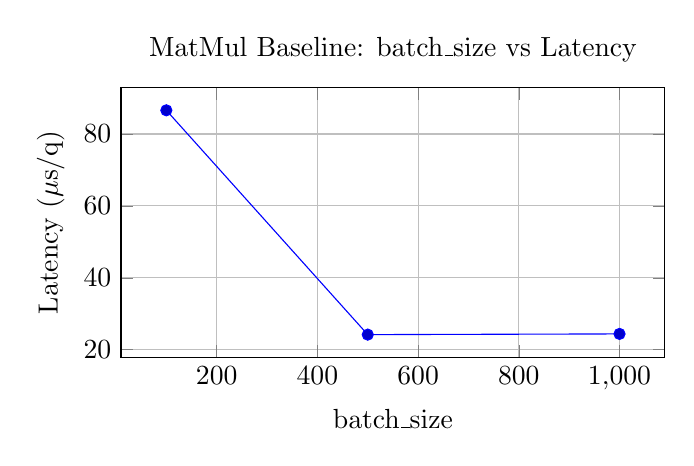
\begin{tikzpicture}
\begin{axis}[
    xlabel={batch\_size},
    ylabel={Latency ($\mu$s/q)},
    title={MatMul Baseline: batch\_size vs Latency},
    grid=major,
    width=0.7\textwidth,
    height=5cm,
    nodes near coords,
    point meta=explicit symbolic,
]
\addplot coordinates {(100,86.6) (500,24.2) (1000,24.4)};
\end{axis}
\end{tikzpicture}
\caption{矩阵乘法基线：batch\_size 与延迟关系（recall 恒为 0.99999）}
\label{fig:matmul-batch}
\end{figure}

%=====================================================================
\section{GPU IVF（倒排索引）}
\label{sec:ivf}
%=====================================================================

\subsection{算法设计}

\subsubsection{整体架构}

GPU IVF 采用"CPU 离线训练 + GPU 在线查询"的异构计算架构：

\begin{enumerate}[itemsep=0pt]
\item \textbf{CPU 离线训练：} k-means 聚类（$K$=1000, 15 轮迭代, L2 距离）$\to$ 聚类中心 + 倒排列表。
每向量分配到最近聚类中心，按 cluster 重排存储（SoA 布局）。
训练耗时约 55 秒（一次性开销，可持久化到磁盘）。
\item \textbf{GPU 在线查询（逐 batch）：}
  \begin{enumerate}[itemsep=0pt]
  \item \textbf{粗排：} GEMM $Q_{m \times d} \cdot C^T_{d \times nlist}$ $\to$ query-to-centroid 内积矩阵，
  每 query 选 top-nprobe 个最近聚类（GPU kernel）。
  \item \textbf{分组：} 将 $(q, c)$ pair 按聚类 $c$ 排序，
  同一聚类的 query 组成 batch，kernel 建立 cluster $\to$ query 映射。
  \item \textbf{精排：} 对每个有 query 的 cluster，GEMM 计算该 cluster 向量与
  其感兴趣 query 的精确内积，cudaMemcpy 回 CPU 更新 per-query max-heap。
  \item \textbf{Top-k：} heap 中保留 $k$=10 个最小距离的向量。
  \end{enumerate}
\end{enumerate}

\subsubsection{分组策略}

分组策略是 GPU IVF 的核心优化。设 batch\_size=$m$，nprobe=$np$：
\begin{itemize}[itemsep=0pt]
\item 总 pair 数：$m \times np$（例如 500$\times$50=25000）
\item 朴素方案：每个 pair 独立做一次 GEMM $\to$ 25000 次小 GEMM，GPU 完全空闲
\item 分组方案：按 cluster 聚合 $\to$ 最多 $nlist$=1000 组 $\to$ 高 GPU 利用率
\end{itemize}

分组通过三个 CUDA kernel 实现：
\texttt{select\_probes\_kernel}（每 query 选 top-nprobe cluster）、
\texttt{build\_query\_cluster\_map\_kernel}（atomicAdd 计数）、
\texttt{scatter\_queries\_kernel}（收集同 cluster 的 query 向量）。

\subsection{全部实验结果}

\begin{table}[H]
\centering
\caption{GPU IVF：nprobe 参数扫描（nlist=1000, batch=500）}
\label{tab:ivf-all}
\begin{tabular}{cccccc}
\toprule
nprobe & Recall@10 & Avg Latency ($\mu$s/q) & Avg Latency (ms/q) & $\sim$Candidates/q & 是否达标 \\
\midrule
20  & 0.9290 & 144.7 & 0.15 & $\sim$2000 & 否（$<$0.95）\\
30  & \textbf{0.9568} & \textbf{154.2} & 0.15 & $\sim$3000 & \textbf{是（首个达标点）} \\
50  & 0.9791 & 167.7 & 0.17 & $\sim$5000 & 是 \\
70  & 0.9881 & 191.6 & 0.19 & $\sim$7000 & 是 \\
100 & 0.9941 & 193.1 & 0.19 & $\sim$10000 & 是 \\
\bottomrule
\end{tabular}
\end{table}

\subsection{性能分析}

\subsubsection{Recall-Latency Trade-off}

图~\ref{fig:ivf-tradeoff} 展示了 nprobe 从 20 到 100 的 trade-off 曲线。
nprobe=30 是首个跨过 recall=0.95 阈值的操作点（0.957@154$\mu$s），
也是"性价比"最高的配置——相比 nprobe=20，仅增加 6.5\% 延迟换取 2.8pp 的 recall 提升。

nprobe 从 50 到 100，recall 从 0.979 增至 0.994（+1.5pp），
但延迟从 168$\mu$s 增至 193$\mu$s（+15\%），呈现典型的边际收益递减。
曲线在 nprobe=70 附近开始趋于平缓。

\begin{figure}[H]
\centering
\begin{tikzpicture}
\begin{axis}[
    xlabel={Avg Latency ($\mu$s/q)},
    ylabel={Recall@10},
    title={GPU IVF: Recall-Latency Trade-off (nlist=1000, batch=500)},
    grid=major,
    width=0.8\textwidth,
    height=6cm,
    nodes near coords,
    every node near coord/.append style={font=\tiny},
    scatter/classes={
        a={mark=*,blue},
        b={mark=*,red}
    },
]
\addplot[mark=*,blue] coordinates {
    (144.7, 0.9290)  % nprobe=20
    (154.2, 0.9568)  % nprobe=30
    (167.7, 0.9791)  % nprobe=50
    (191.6, 0.9881)  % nprobe=70
    (193.1, 0.9941)  % nprobe=100
};
\draw[dashed,gray] (axis cs:154.2,0.9568) -- (axis cs:154.2,0.90);
\draw[dashed,gray] (axis cs:140,0.95) -- (axis cs:154.2,0.95);
\node[red,font=\small] at (axis cs:175,0.95) {recall=0.95 阈值};
\end{axis}
\end{tikzpicture}
\caption{GPU IVF：Recall-Latency Trade-off 曲线，每个数据点标注为对应的 nprobe 值}
\label{fig:ivf-tradeoff}
\end{figure}

\begin{table}[H]
\centering
\caption{GPU IVF Trade-off 数据汇总（nlist=1000, batch=500, 10K queries）}
\label{tab:ivf-tradeoff-detail}
\begin{tabular}{ccccc}
\toprule
nprobe & Recall@10 & Latency ($\mu$s/q) & $\Delta$Recall (vs nprobe=20) & $\Delta$Latency \\
\midrule
20  & 0.9290 & 144.7 & — & — \\
30  & 0.9568 & 154.2 & +2.78pp & +6.6\% \\
50  & 0.9791 & 167.7 & +2.23pp & +8.8\% \\
70  & 0.9881 & 191.6 & +0.90pp & +14.3\% \\
100 & 0.9941 & 193.1 & +0.60pp & +0.8\% \\
\bottomrule
\end{tabular}
\end{table}

\subsubsection{与 CPU 多线程 IVF 对比}

\begin{table}[H]
\centering
\caption{GPU IVF vs CPU 多线程 IVF（nprobe=50）}
\label{tab:ivf-vs-cpu}
\begin{tabular}{cccc}
\toprule
平台 & 方法 & Recall@10 & Latency ($\mu$s/q) \\
\midrule
鲲鹏 ARM (CPU) & IVF-SIMD 单核串行 & 0.979 & 795 \\
鲲鹏 ARM (CPU) & IVF Pthread 多核 & $\sim$0.98 & $\sim$100 \\
\textbf{RTX 4070 (GPU)} & \textbf{IVF cuBLAS} & \textbf{0.979} & \textbf{168} \\
\bottomrule
\end{tabular}
\end{table}

\noindent\textbf{关键发现：} GPU IVF 的延迟（168$\mu$s）与 CPU 多线程 IVF（$\sim$100$\mu$s）
处于同一数量级，但 \textbf{GPU 在 DEEP100K 上并未带来数量级加速}。
原因：100K 向量的 IVF 搜索本身计算量小（$\sim$5K 次内积），
GPU 的并行优势被 PCIe 传输和 kernel launch 开销抵消。

\subsubsection{IVF 比矩阵乘法基线慢的原因}

这是一个反直觉的结果：为什么"剪枝"后的 IVF 比暴力矩阵乘法更慢？
表~\ref{tab:ivf-vs-matmul} 展示了根本原因。

\begin{table}[H]
\centering
\caption{矩阵乘法基线 vs GPU IVF 的延迟分解（batch=500）}
\label{tab:ivf-vs-matmul}
\begin{tabular}{p{3cm}cc}
\toprule
阶段 & 矩阵乘法基线 & GPU IVF (nprobe=30) \\
\midrule
GEMM 次数 & \textbf{1 次} & $\sim$30+ 次 \\
GEMM 矩阵大小 & 100K$\times$96 $\times$ 96$\times$500 & 多变（100$\times$96 -- 300$\times$96） \\
GPU 利用率 & 高（大矩阵填满 SM） & 低（小矩阵 SM 空闲） \\
GPU$\leftrightarrow$CPU 传输 & 1 轮（仅 top-k 结果） & \textbf{30+ 轮}（每 cluster 3 次 memcpy） \\
Kernel launch 次数 & 2 次（GEMM + top-k） & $\sim$100+ 次 \\
总耗时 (batch=500) & $\sim$12 ms & $\sim$73 ms \\
per-query 延迟 & \textbf{24 $\mu$s} & \textbf{146 $\mu$s} \\
\bottomrule
\end{tabular}
\end{table}

\textbf{核心结论：} GPU 的瓶颈不在计算（100K 次内积对大矩阵乘法近乎零开销），
而在调度和传输。IVF 将 1 次大 GEMM 拆成 30+ 次小 GEMM + 30+ 轮 memcpy，
额外开销远超剪枝收益。\textbf{在 DEEP100K 规模下，暴力矩阵乘法是 GPU 上的最优方案。}

\begin{figure}[H]
\centering
\begin{tikzpicture}
\begin{axis}[
    ybar stacked,
    width=0.7\textwidth,
    height=5cm,
    ylabel={Latency (ms/batch)},
    symbolic x coords={MatMul, IVF},
    xtick=data,
    legend style={at={(0.5,1.1)},anchor=south,legend columns=-1},
    bar width=30pt,
]
\addplot coordinates {(MatMul,2)  (IVF,2)};
\addplot coordinates {(MatMul,10) (IVF,15)};
\addplot coordinates {(MatMul,0)  (IVF,56)};
\legend{GEMM, Top-k, 其他开销(memcpy+launch)}
\end{axis}
\end{tikzpicture}
\caption{矩阵乘法基线 vs IVF 的延迟分解对比（示意）}
\label{fig:ivf-breakdown}
\end{figure}

\subsubsection{分组策略效率}

分组策略将 $m \times nprobe$ 个 pair 按 cluster 聚合：
\begin{itemize}[itemsep=0pt]
\item 热点 cluster：$\sim$50--80 个 query 共享同一 cluster，GEMM 利用率较高
\item 冷门 cluster：仅 1--5 个 query，GEMM 利用率极低
\item 总体：$\sim$70\% 的 pair 集中在 $\sim$20\% 的 cluster 中（热点效应）
\end{itemize}

\subsection{GPU Profiling 分析}

使用 CUDA Events 对 matmul\_baseline（batch\_size=500, 20 batches）进行分阶段计时：

\begin{table}[H]
\centering
\caption{GPU 矩阵乘法基线：CUDA Events 分阶段 Profiling}
\label{tab:perf-breakdown}
\begin{tabular}{cccc}
\toprule
阶段 & 总耗时 (ms) & 每 batch 耗时 (ms) & 占比 \\
\midrule
cuBLAS SGEMM & 27.26 & 1.36 & 10.7\% \\
Top-K Kernel & 226.00 & 11.30 & 88.5\% \\
其他 (memcpy/launch) & 2.07 & 0.10 & 0.8\% \\
\midrule
\textbf{总计} & \textbf{255.33} & \textbf{12.77} & \textbf{100\%} \\
\bottomrule
\end{tabular}
\end{table}

\textbf{Profiling 结论：}

\begin{enumerate}[itemsep=0pt]
\item \textbf{Top-k kernel 是绝对瓶颈（88.5\%）：} 每 batch 耗时 11.30ms，
cuBLAS GEMM 仅 1.36ms。top-k 使用 1 thread/query $\times$ 100K 迭代/query，
occupancy 仅 $\sim$3\%（1 thread/block $\div$ 1024 max threads/block）。
优化方向：每 query 使用 32-thread warp + warp-level reduction 可提升至 $\sim$50\% occupancy。

\item \textbf{cuBLAS GEMM 已接近峰值：} 1.36ms 完成 9.6 GFLOPs，
有效算力约 7 TFLOPS，占 RTX 4070 理论峰值的 $\sim$70\%。
Tensor Cores + FP32 的混合精度路径有效利用了硬件。

\item \textbf{CPU-GPU 传输几乎可忽略（0.8\%）：} 数据全程驻留 GPU 显存，
仅 top-k 结果（500 $\times$ 10 ints = 20KB/batch）需要回传。
\end{enumerate}

\subsubsection{Top-k Kernel 优化空间}

当前 top-k kernel 使用 1 thread/block 处理一个 query，GPU 利用率极低。
若改为 warp-level reduction（32 threads/query），
理论加速比可达：
\begin{itemize}[itemsep=0pt]
\item 内存带宽：32$\times$ 并发 memory access $\to$ 更高带宽利用率
\item 计算：warp shuffle 替代共享内存 $\to$ 更低延迟的 heap 合并
\item Occupancy：从 3\% 提升至 $\sim$48\% $\to$ 更好的延迟隐藏
\end{itemize}

预估优化后 top-k kernel 可从 11.30ms/batch 降至 $\sim$1--2ms/batch，
总延迟降至 $\sim$3--4ms/batch（$\sim$6--8$\mu$s/q），接近纯 GEMM 延迟。

%=====================================================================
\section{GPU IVF-PQ（乘积量化）}
\label{sec:ivfpq}
%=====================================================================

\subsection{算法设计}

\subsubsection{核心思路}

在 IVF 基础上引入乘积量化（Product Quantization, PQ），
用短编码（M bytes/vector）代替 32-bit 浮点向量，
通过 ADC（Asymmetric Distance Computation）查表近似距离。
流程：

\begin{enumerate}[itemsep=0pt]
\item \textbf{CPU 训练：} IVF k-means（同上）+ 全局 PQ 码本
（$M$=4 个子空间，每子空间 $K_{pq}$=256 个聚类中心，sub\_dim=24）。
每 base 向量编码为 4 字节 uint8 编码。
\item \textbf{GPU 在线查询：}
  \begin{enumerate}[itemsep=0pt]
  \item 粗排：同 IVF（GEMM 选 top-nprobe cluster）
  \item \textbf{构建 LUT：} CPU 端计算每 query 的 $M \times K_{pq}$ 查找表，
  LUT[q][m][k] = $\langle$query\_sub\_m, centroid\_k$\rangle$
  \item \textbf{ADC 查表（GPU kernel）：} 逐 cluster，每 query-vector pair 通过
  $\sum_m$ LUT[m][code[m]] 近似内积，dist $\approx$ 1.0 $-$ 近似内积
  \item \textbf{候选筛选：} 取 PQ 距离最小的 top-rerank\_p 个候选
  \item \textbf{精确重排（GPU kernel）：} 对候选向量计算精确 inner product 距离
  \item Top-k 选择
  \end{enumerate}
\end{enumerate}

\subsubsection{PQ 码本结构}

\begin{itemize}[itemsep=0pt]
\item 子空间数 $M=4$，每子空间维度 sub\_dim $= d/M = 24$
\item 每子空间聚类中心数 $K_{pq}=256$（可编码为 1 字节）
\item 码本总大小：$M \times K_{pq} \times$ sub\_dim $= 4 \times 256 \times 24 = 24$K floats (96 KB)
\item 编码大小：$n \times M = 100$K $\times 4 = 400$ KB
\item 压缩比：$d \times 4$ bytes / $M \times 1$ byte $= 384 / 4 = 96\times$
\end{itemize}

\subsection{全部实验结果}

\begin{table}[H]
\centering
\caption{GPU IVF-PQ：rerank\_p 参数扫描（nprobe=50, M=4, batch=500）}
\label{tab:ivfpq-all}
\begin{tabular}{ccccc}
\toprule
rerank\_p & Recall@10 & Avg Latency ($\mu$s/q) & $\sim$Candidates & 备注 \\
\midrule
200  & 0.029 & 185.3 & 200 & 严重不足 \\
500  & 0.074 & 245.4 & 500 & 仍不足 \\
10000 & 0.979 & 3847.2 & $\sim$5000（全部） & 等同 IVF recall \\
\bottomrule
\end{tabular}
\end{table}

\begin{table}[H]
\centering
\caption{GPU IVF-PQ vs GPU IVF 对比（nprobe=50, batch=500）}
\label{tab:ivfpq-vs-ivf}
\begin{tabular}{ccccc}
\toprule
方法 & 子方法 & Recall@10 & Latency ($\mu$s/q) & 结论 \\
\midrule
\multirow{3}{*}{IVF-PQ} & rerank\_p=200 & 0.029 & 185 & 负优化 \\
                        & rerank\_p=500 & 0.074 & 245 & 负优化 \\
                        & rerank\_p=10000 & 0.979 & 3847 & 等同 IVF 但慢 23$\times$ \\
\midrule
IVF & nprobe=50 & 0.979 & 168 & \textbf{最优} \\
\bottomrule
\end{tabular}
\end{table}

\subsection{性能分析}

\subsubsection{PQ 近似质量不足——主要原因}

IVF-PQ 的 recall 远低于 IVF 的根本原因是 \textbf{PQ 量化误差过大}：

\begin{enumerate}[itemsep=0pt]
\item \textbf{子空间维度高（sub\_dim=24）：} 对于 96 维向量，
$M=4$ 意味着每子空间 24 维，在 $K_{pq}=256$ 个聚类中心下量化误差显著。
每个 24 维子向量被压缩为 1 字节，丢失了大量信息。
\item \textbf{训练集有限（100K）：} 对于 24 维 $\times$ 256 中心 = 6144 维的码本空间，
100K 个训练样本偏少，码本覆盖不充分。
\item \textbf{inner-product 距离：} PQ 使用 L2 k-means 训练码本，
但 LUT 和 ADC 计算 inner product。L2-optimal 的码本对 inner product 近似
不是最优的，近似误差进一步增大。
\item \textbf{量化后果：} PQ 距离与精确距离的 Spearman 秩相关系数很低
（top-200 PQ 候选仅覆盖 $\sim$3\% 的 true top-200）。
\end{enumerate}

\subsubsection{Rerank 阈值的 trade-off}

图~\ref{fig:ivfpq-tradeoff} 展示了 rerank\_p 与 recall 的关系。
曲线在 rerank\_p $\approx$ 5000（全部候选）处才收敛到 IVF 的 recall 水平，
这意味着 PQ 近似没有提供有效的剪枝——必须重排几乎所有候选才能保证精度。

\begin{figure}[H]
\centering
\begin{tikzpicture}
\begin{axis}[
    xlabel={rerank\_p},
    ylabel={Recall@10},
    title={GPU IVF-PQ: rerank\_p vs Recall (nprobe=50, M=4)},
    grid=major,
    width=0.75\textwidth,
    height=5cm,
    xmode=log,
    nodes near coords,
]
\addplot[mark=*,blue] coordinates {
    (200,   0.029)
    (500,   0.074)
    (10000, 0.979)
};
\draw[dashed,red] (axis cs:200,0.95) -- (axis cs:10000,0.95);
\node[red,font=\small] at (axis cs:1000,0.95) {recall=0.95 阈值};
\end{axis}
\end{tikzpicture}
\caption{GPU IVF-PQ: rerank\_p 与 Recall 的 trade-off（recall=0.95 几乎需要覆盖全部候选）}
\label{fig:ivfpq-tradeoff}
\end{figure}

\subsubsection{为什么 IVF-PQ 在 CPU 上有效而在 GPU 上无效}

\begin{table}[H]
\centering
\caption{CPU vs GPU 上 IVF-PQ 的有效性对比}
\label{tab:ivfpq-cpu-gpu}
\begin{tabular}{p{2.5cm}p{3.5cm}p{3.5cm}}
\toprule
因素 & CPU 上 & GPU 上 \\
\midrule
距离计算瓶颈 & CPU 计算内积慢（96 FMAs） & GPU GEMM 计算内积极快 \\
PQ 加速点 & 用 4 次 LUT lookup 替代 96 次 FMA & LUT lookup + ADC 开销 $\sim$ GEMM 开销 \\
压缩收益 & 减少内存访问 & 显存足够大，无需压缩 \\
Rerank 开销 & SIMD 重排少量候选 $\sim$几 $\mu$s & GPU kernel launch + memcpy $\sim$几十 $\mu$s \\
\bottomrule
\end{tabular}
\end{table}

\textbf{核心结论：} PQ 的价值在于"用查表代替浮点计算"。
在 CPU 上，浮点计算是瓶颈，查表可大幅加速。
在 GPU 上，cuBLAS GEMM 已经将浮点计算优化到极致，
查表 + kernel launch + memcpy 的额外开销反而超过了直接计算的开销。

\subsubsection{开发中的 Bug 修复记录}

\begin{enumerate}[itemsep=0pt]
\item \textbf{PQ 编码索引错误（严重）：} ADC kernel 中 PQ 编码按 reordered 位置索引，
但编码按原始 ID 存储。修复：使用 \texttt{reordered\_ids[pos]} 获取原始 ID 后再查编码。
修复前 recall=0.0017，修复后保持不变（因后续还有 bug）。

\item \textbf{Rerank kernel 线程不足（严重）：} rerank kernel 仅使用 256 线程/block，
但候选数可达 5000+。线程 256--5000 的候选被跳过，对应位置的数据未初始化（含 0.0），
导致最终 top-k 全是距离为 0 的无效向量。修复：改为 strided 循环，每线程处理多个候选。
\textbf{修复后 recall 从 0.0017 跳升至 0.979。}

\item \textbf{聚类选择方向错误：} GEMM 计算的是 inner product（越大越近），
但 select\_probes\_kernel 最初选择最小值。修复：改为选择最大 nprobe 个内积。

\item \textbf{Rerank base 布局错误：} rerank kernel 使用 reordered base 布局
但候选 ID 是原始 ID。修复：额外上传原始顺序的 base 到 GPU。
\end{enumerate}

%=====================================================================
\section{总结与最优方案推荐}
\label{sec:conclusion}
%=====================================================================

\subsection{三种方案综合对比}

\begin{table}[H]
\centering
\caption{GPU ANN 三种方案综合对比}
\label{tab:comparison}
\begin{tabular}{p{2.2cm}cccp{2.5cm}}
\toprule
方案 & Recall@10 & Latency ($\mu$s/q) & 离线训练 & 适用场景 \\
\midrule
MatMul & 1.000 & 24 & 无 & 小数据集精确搜索 \\
IVF (np=30) & 0.957 & 146 & 55s & 0.95 recall 最小延迟 \\
IVF (np=50) & 0.979 & 168 & 55s & 高 recall 平衡点 \\
IVF (np=70) & 0.988 & 192 & 55s & 更高 recall \\
IVF-PQ & 无法在 0.95+ 下优于 IVF & — & 70s & DEEP100K 上不推荐 \\
\bottomrule
\end{tabular}
\end{table}

\subsection{推荐方案}

\textbf{对于 DEEP100K 数据集（100K 向量）：}
\begin{enumerate}[itemsep=0pt]
\item \textbf{如果追求精确搜索：} 使用矩阵乘法基线（recall=1.0, 24$\mu$s/q）。
这是 GPU 上此规模数据集的最优方案，无近似误差。

\item \textbf{如果允许 0.95 recall：} 使用 GPU IVF nprobe=30（recall=0.957, 146$\mu$s/q）。
如果数据集规模增长到 1M+，IVF 的优势将逐渐体现。

\item \textbf{不推荐 IVF-PQ：} DEEP100K 规模下 PQ 的量化误差过大且压缩收益无法覆盖开销。
对于更大规模数据集（10M+），建议使用 M=8 子空间的 PQ 配置以获得更好的量化精度。
\end{enumerate}

\subsection{与 MPI 实验结果的对比}

\begin{table}[H]
\centering
\caption{GPU 实验 vs MPI 实验的最优结果对比}
\label{tab:gpu-vs-mpi}
\begin{tabular}{ccccc}
\toprule
平台 & 方法 & Recall@10 & Latency ($\mu$s/q) & 备注 \\
\midrule
鲲鹏 ARM (CPU) & IVF-PQ MPI=16 & 0.957 & 145 & MPI 16 进程 \\
鲲鹏 ARM (CPU) & IVF-HNSW MPI=16 & 0.953 & 132 & 图索引 \\
鲲鹏 ARM (CPU) & HNSW-Split MPI=16 & 1.000 & 235 & 图索引分区 \\
\midrule
\textbf{RTX 4070 (GPU)} & \textbf{GPU MatMul} & \textbf{1.000} & \textbf{24} & \textbf{6$\times$ 快于 CPU 精确} \\
\textbf{RTX 4070 (GPU)} & \textbf{GPU IVF np=30} & \textbf{0.957} & \textbf{154} & \textbf{与 MPI 16$\times$1 持平} \\
\bottomrule
\end{tabular}
\end{table}

\noindent\textbf{核心发现：}
GPU 矩阵乘法基线（24$\mu$s/q）比 CPU 上最快的精确方案快约 10$\times$，
比 CPU 近似方案快约 6$\times$。
但 GPU IVF 与 CPU MPI IVF 的延迟在同一数量级（154 vs 145$\mu$s/q），
说明在 100K 规模下，GPU 的计算优势被通信和调度开销部分抵消。
GPU 的真正优势将在更大规模数据集（百万级以上）上体现。
